\subsection{Drone Parrot Bebop 2}

Le modèle du drone utilisé dans le cadre de notre projet STL est un drone \textit{Parrot BEBOP 2}\footnote{\url{https://www.parrot.com/fr/Drones/Parrot-Bebop-2}}. Parmi ses spécifications techniques, on peut relever :
\begin{itemize}
\item un poids de 500g
\item une autonomie de 25min
\item 4 hélices flexibles motorisées
\item une vitesse de pointe de 60km/h en horizontal et de 21km/h en vertical
\item une caméra Full HD permettant de filmer et photographier
\item un GPS pour le contrôle de vol et le dispositif de suivi/retour automatique
\item une antenne  Wi-Fi émettant un signal jusqu'à 300m
\end{itemize}

\newpage
\begin{figure}
\begin{center}
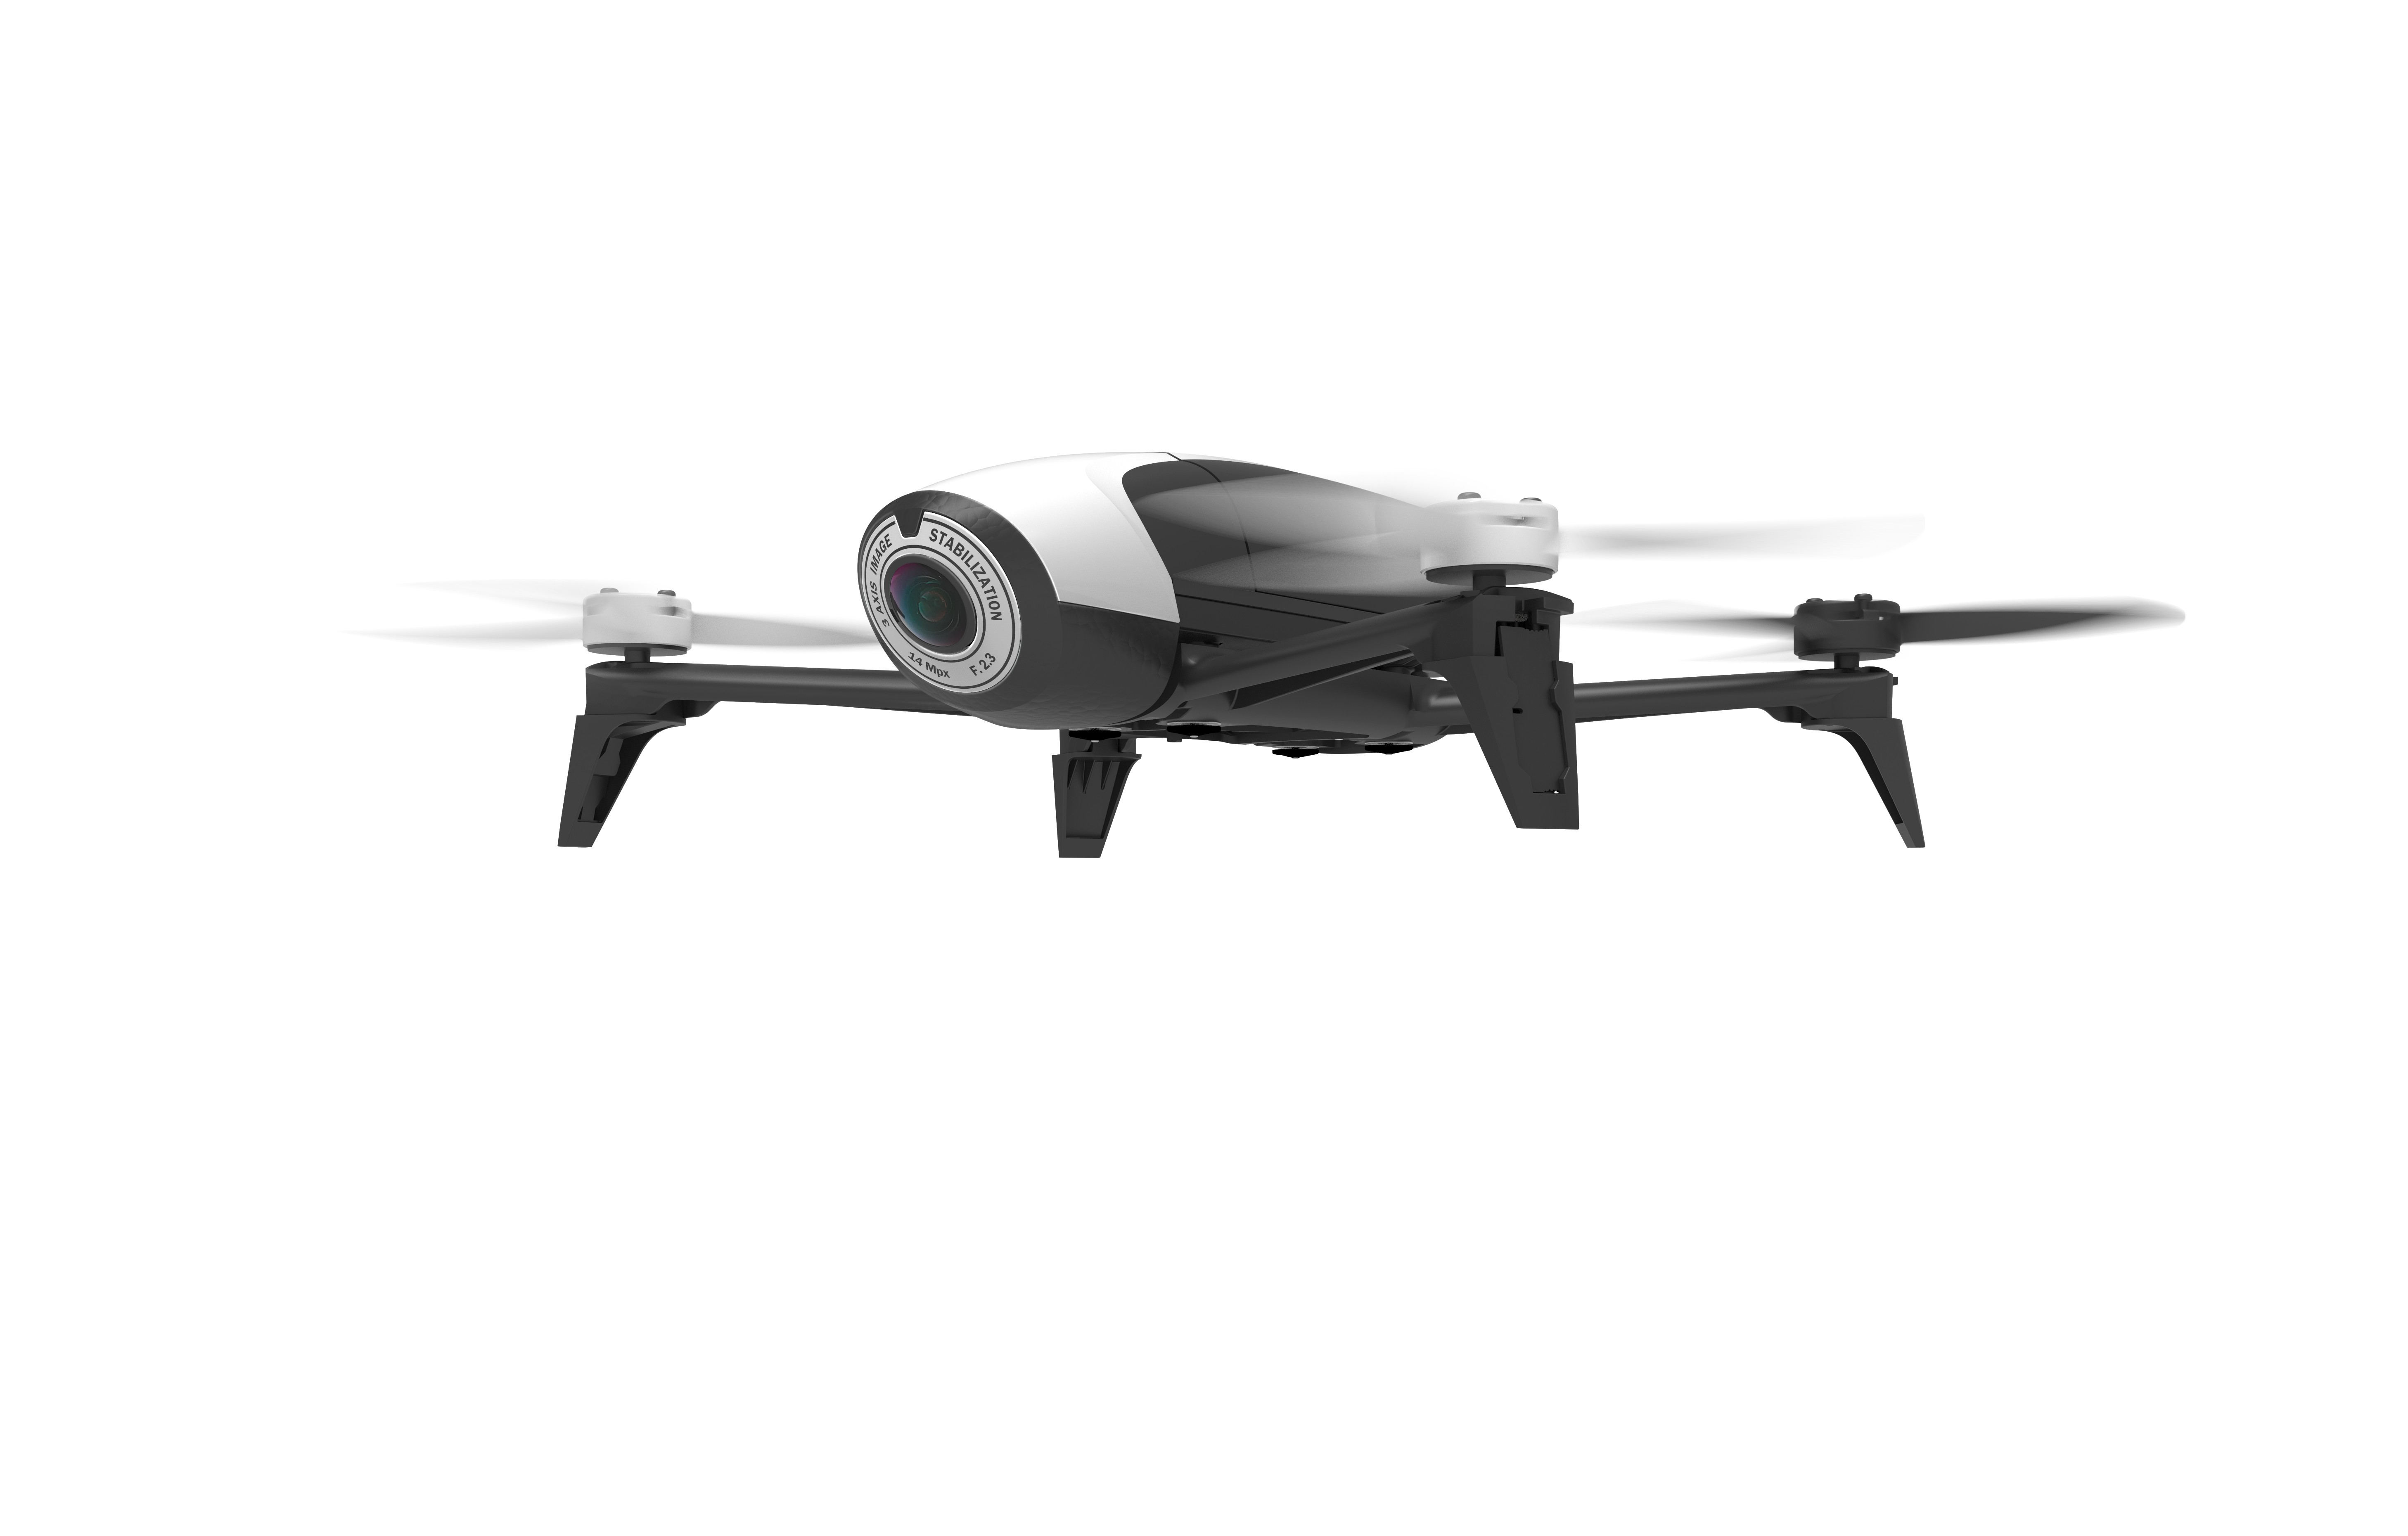
\includegraphics[scale=0.05]{images/drone.jpg}
\caption{Drone Parrot BEBOP 2}
\end{center}
\end{figure}

Une application fournie par le constructeur appelée \textit{Free Flight Pro} permet de piloter l'appareil via un smartphone sous \android{} ou \textit{iOS} connectée à travers son propre réseau Wi-Fi. De nombreuses fonctionnalités sont proposées par l'application en plus des commandes de contrôle du drone comme la possibilité de faire des figures prédéfinis ou de partager ses données de navigation avec d'autres pilotes.

\paragraph{}
En ce qui concerne le développement du programme du drone, nous nous sommes servis de la version 3 de la SDK mise à disposition\footnote{\url{https://github.com/Parrot-Developers/arsdk_manifests.git}} avec pour documentation quelques programmes exemple et un forum de développeurs.